% !TeX document-id = {3c9fb181-ef8d-46f4-a369-f483876e4c37}
% !TeX TXS-program:compile = txs:///pdflatex/[--shell-escape]


\documentclass[fleqn,11pt,aspectratio=169]{beamer}
\usepackage{tubslogo}
\usepackage{amsmath}
\usepackage{amsfonts}
\usepackage{amssymb}
\usepackage{graphicx}
\usepackage{qrcode}
\usepackage{geometry}
\usepackage{tikz}
\usepackage{amsthm}
\usepackage{float}
\usepackage{cleveref}
\usepackage{acronym}
\usepackage{algpseudocode}

\usepackage{fancyvrb}
\usepackage{fvextra}
\usepackage[normalem]{ulem}
\usepackage{enumerate}

\usepackage[overload]{textcase}
\usepackage{minitoc}        
%\usepackage{etoc}        
\usepackage{printlen}
\usepackage{url}  
\usepackage{tabularx}  
\usepackage{soul}
\usepackage{siunitx}
\usepackage{eqparbox}
\sisetup{
	per-mode=symbol,
}
\usepackage[utf8]{inputenc}
\usepackage[
	backend=biber,
	style=numeric,
]{biblatex}
\addbibresource{bibfile.bib}

\usepackage[rgb,dvipsnames]{xcolor}

\selectcolormodel{natural}
\usepackage{ninecolors}
\selectcolormodel{rgb}
\usepackage{tabularray}
\usepackage{minted}
\usemintedstyle{emacs,tabsize=2,linenos,xleftmargin=10pt,highlightcolor=cyan}

\usepackage[export]{adjustbox}% http://ctan.org/pkg/adjustbox

\usepackage[append]{beamersubframe}
\usepackage[american]{babel}
\usepackage{graphicx}
\setbeamerfont{normal text}{size=12pt}

\date{July 16, 2026}
\usetheme[%
  %nexus,%        Nexus Fonts benutzen
  %lnum,%         Versalziffern verwenden
  %cmyk,%<rgbprint>,          Auswahl des Farbmodells
  blue,%<orange/green/violet> Auswahl des Sekundärfarbklangs
  dark,%<light,medium>        Auswahl der Helligkeit
  %colorhead,%    Farbig hinterlegte Kopfleiste
  %colorfoot,%    Farbig hinterlegt Fußleiste auf Titelseite
  colorblocks,%   Blöcke Farbig hinterlegen
  %nopagenum,%    Keine Seitennumer in Fußzeile
  %nodate,%       Kein Datum in Fußleiste
  tocinheader,%   Inhaltsverzeichnis in Kopfleiste
  %tinytocinheader,% kleines Kopfleisten-Inhaltsverzeichnis
  %widetoc,%      breites Kopfleisten-Inhaltsverzeichnis
  %narrowtoc,%    schmales Kopfleisten-Inhaltsverzeichnis
  %nosubsectionsinheader,%  Keine subsections im Kopfleisten-Inhaltsverzeichnis
  %nologoinfoot,% Kein Logo im Fußbereich darstellen
  ]{tubs}
% Titelseite
\title{Algorithm Engineering 2026: Sheet 06 - Exam Prep}
\author{Rouven Kniep}

%titlepage font and background
\setbeamercolor{titlebarfirst}{parent=titlepage, bg=titlepage.bg!0}

% Edit the TUBS template to move the tubslogo into place for the title
\let\tubslogoAbsOld\tubslogoAbs
\renewcommand{\tubslogoAbs}[1]{\raisebox{-2.3mm}{\tubslogoAbsOld{#1}}}

% Quoteblock 
\newcommand{\quotebox}[1]{\begin{center}\fcolorbox{white}{blue!15!gray!15}{\begin{minipage}{0.9\linewidth}\vspace{10pt}\center\begin{minipage}{0.8\linewidth}{\space\Huge``}{#1}{\hspace{1.5em}\break\null\Huge\hfill''}\end{minipage}\smallbreak\end{minipage}}\end{center}}

% smaller highlighting
\makeatletter
\def\SOUL@hlpreamble{%
	\setul{}{1.5ex}%         !!!change this value!!! default is 2.5ex
	\let\SOUL@stcolor\SOUL@hlcolor
	\SOUL@stpreamble
}
\makeatother

% Hline with padding
\UseTblrLibrary{booktabs}
\NewTableCommand{\phline}{\specialrule{.4pt}{2pt}{2pt}}

\begin{document}

\part{main}
\begin{frame}[plain]
	\titlepage
\end{frame}	


\section{Ex1 - CPU Arch + Perf Engineering}

\begin{frame}[t]{1a: Array of Structures vs Structure of Arrays}
	\only<1,6>{
	\begin{block}{}
		Describe the terms ‘array of structures’ and ‘structure of arrays’ in your own words and the benefits and drawbacks of each.
	\end{block}
	}
	\only<2>{
		\centering
		Scalar Pipeline (example addition): 
		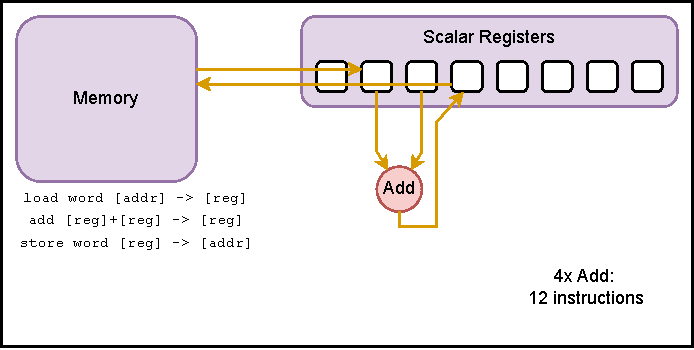
\includegraphics[keepaspectratio, height=0.8\textheight, page=1, trim={3pt 3pt 3pt 3pt}, clip]{simd.pdf}
	}
	\only<3>{
		\centering
		SIMD Pipeline (example addition):
		\includegraphics[keepaspectratio, height=0.8\textheight, page=2, trim={3pt 3pt 3pt 3pt}, clip]{simd.pdf}
	}
	
	\only<4>{
		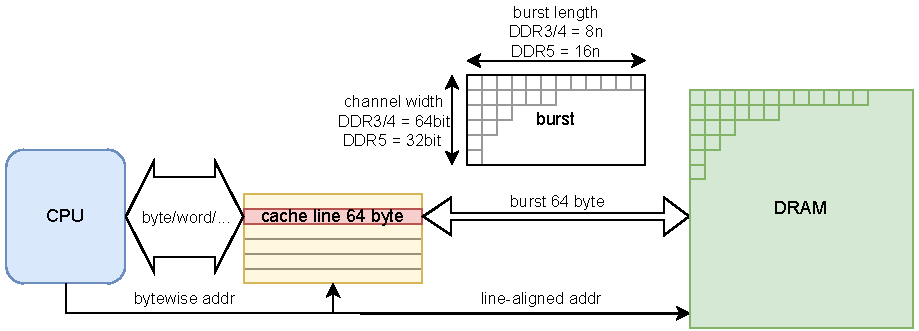
\includegraphics[keepaspectratio, width=\textwidth]{../S02/CPU_memory_cachelines.pdf}
		
		(recap from S02)
	}
	\only<5>{
	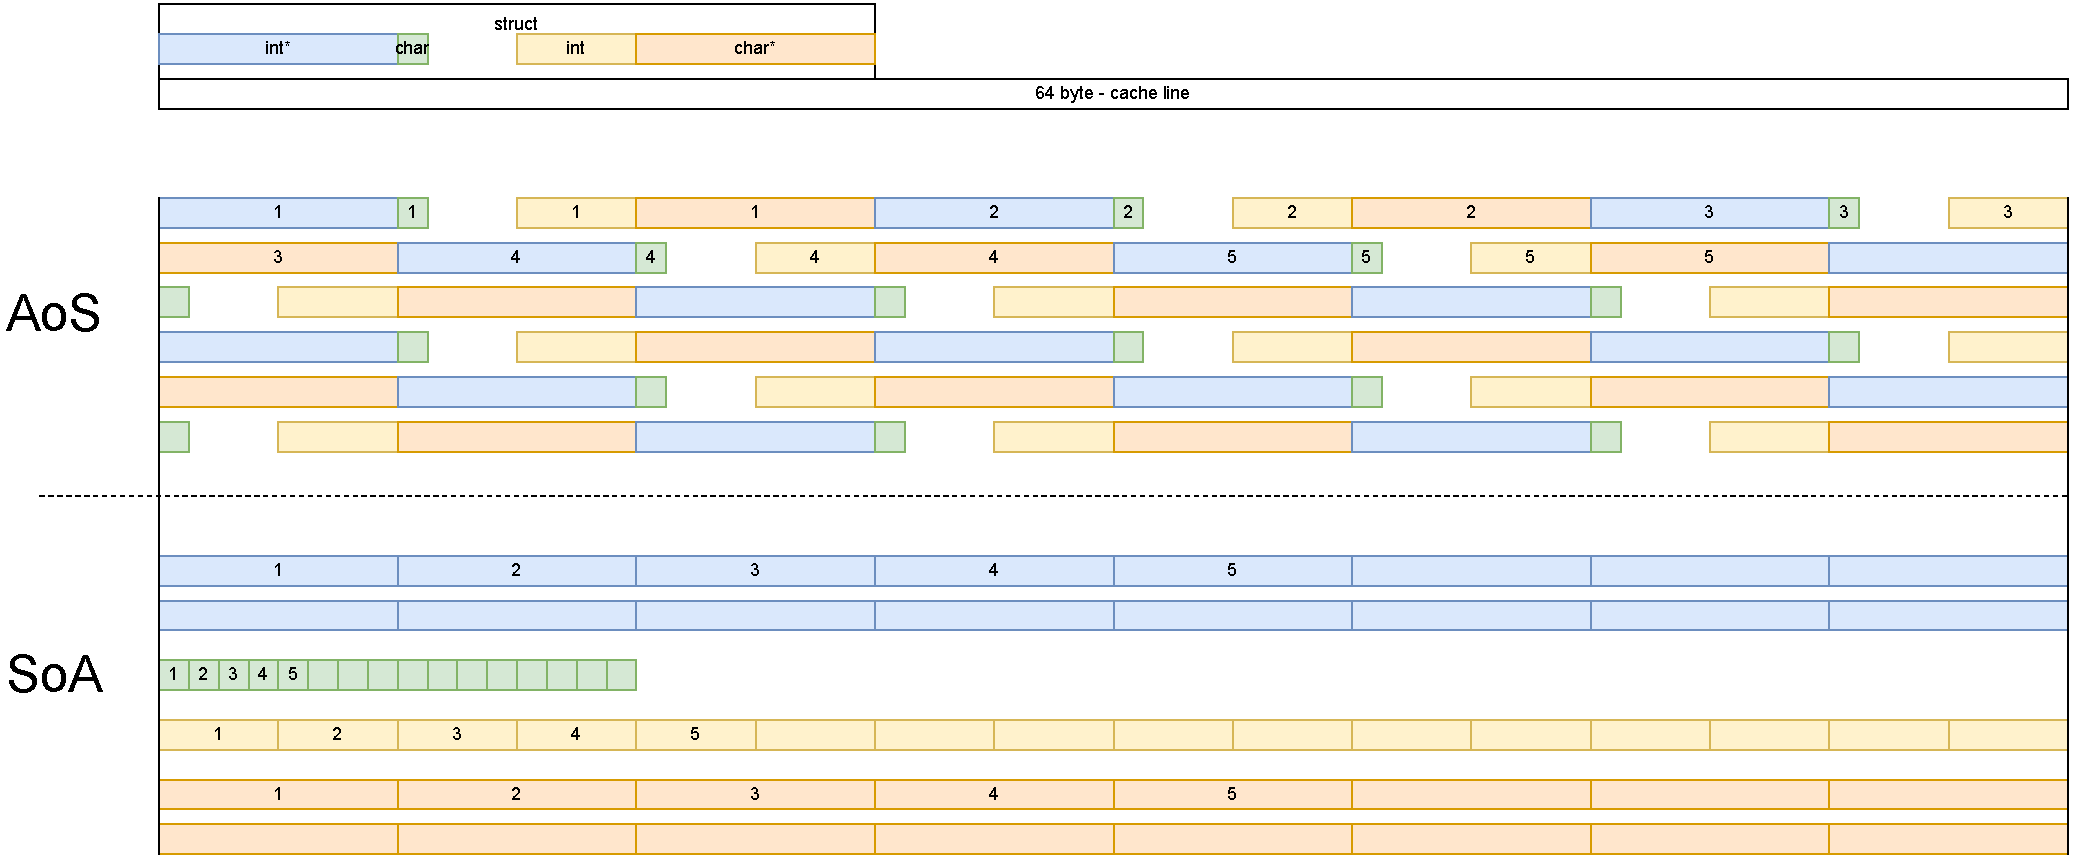
\includegraphics[keepaspectratio, width=\textwidth]{aossoa.pdf}
	}
	\only<6>{
		\vspace{10pt}
		\begin{columns}[T]
			\column{0.45 \textwidth}
			\textbf{Array of Structures}: structs put one after another into the array
			\begin{itemize}
				\item natural to programmers (OOP)
				\item can easily + efficiently interface indivial objects
				\item edge case: good for 2d/3d/4d specialized instruction dot products
			\end{itemize}
			\column{0.45 \textwidth}
			\textbf{Structure of Arrays}: seperate struct members into parallel arrays per member
			\begin{itemize}
				\item when iterating over single/few members: improved efficiency of memory bandwidth and cache
				\item compiler can auto-vectorize code for SIMD
				\item slightly less memory useage
			\end{itemize}
		\end{columns}
	}	
\end{frame}

\begin{frame}[t]{1b: Parallel Solvers}
	\begin{block}{}
		When solving hard problems, what simple approach to parallelization can often be surprisingly (and embarrassingly) competitive with complex, parallelized solvers?
	\end{block}
	\begin{columns}[T]
		\column{0.4\textwidth}
		\only<2,3>{
		\textbf{Multithreaded Portfolio Solvers}:
			\begin{itemize}
				\item different cheap single-threaded heuristics
				\item multiple attempts with different parameters \& random seeds
				\item run several in parallel
				\item return best solution
			\end{itemize}
		}
		\column{0.5\textwidth}
		\only<3>{
			Drawbacks \& Benefits
			\begin{itemize}
				\item typically different heuristics $\implies$ fast
				\item different approaches $\implies$ usually good
				\item little data sharing $\implies$
				\begin{itemize}
					\item little inter-process communication
					\item poor L3 cache hit rate \& potential memory data rate bottleneck
					\item large RAM required 
				\end{itemize}
				\item typically bad bounds (if any)
			\end{itemize}
		}
	\end{columns}
\end{frame}

\begin{frame}[t]{1c: Amdahl's Law}
	\begin{block}{}
		State Amdahl’s Law and explain what it implies for where you should spend optimization effort.
	\end{block}
	\only<2,3>{
		\begin{columns}[T]
			\column{0.45\textwidth}
			$S_{overall} = \frac{t_{old}}{t_{optimized}} = \frac{1}{(1-f_{section})+\frac{f_{section}}{S_{section}}}$
			
			\vspace{8pt}
			
			$f$ fraction of old runtime; \\
			$S$ Speedup; $t$ runtime;
	
			\column{0.45\textwidth}	
			the overall performance improvement gained by optimizing a single part of a system is limited by the fraction of time that the improved part is actually used. \cite{REDDY2011209}		
		\end{columns}
	}	
	\vspace{10pt}
	\only<3>{	
		\begin{center}
			Don't optimize what looks bad, instead \textbf{measure and optimize} where it matters!
			
			Optimizing 10\% by 10$\times$ is less relevant than optimizing 60\% by 1.3$\times$
		\end{center}	
	}
\end{frame}

\begin{frame}[t]{1d: Profiler Families}
	\begin{block}{}
		Profiling tools fall into two big families. Name both, describe each mechanism, and give the main trade-off
	\end{block}
	\only<2>{
		\begin{columns}[T]
			\column{0.45\textwidth}
			Sampling
			\begin{itemize}
				\item interrupt program at regular intervals
				\item then record info (call stack, branch \& cache misses, \dots)
				\item aggregate info into stochastic profile
				\item cannot get per-line infos (execution time, branching, cache, ..)
				\item may miss very small functions 
				\item cannot measure test coverage
			\end{itemize}			
			
			\column{0.45\textwidth}	
			Instrumentation
			\begin{itemize}
				\item change program execution (emulation or inserting monitoring code)
				\item attach any measurement instrument
				\item non-uniformly alters execution time (large monitoring overhead)
				\item skews measurements (cache \& branch hit rate worsens)
				\item $\implies$ bad for performance analysis
			\end{itemize}			
		\end{columns}
	}	
\end{frame}


\section{Ex2 - Data Structures + Optimization Fundamentals}

\begin{frame}[t]{2a: Union-Find in Theory \& Practice}
	\begin{block}{}
		State the theoretical amortized complexity of Union-Find (find/unite) with union-by-rank + path compression, and the complexity to assume in practice. Justify.
	\end{block}

	Background: data structure for storing a partition, see Lecture 04.

	\only<2>{
		\begin{itemize}
			\item theory: $\mathcal{O}(\alpha(n))$ \textbf{amortized}, with $\alpha$ = inverse Ackermann Function
			\begin{itemize}
				\item $\alpha(n) \leq 5 \hspace{8pt} \forall n\in \mathcal{N} \mid n \le 10^{80}$ (which is basically constant)
				\item one $\mathcal{O}(n)$ array $\implies$ little data: $10^7$ elements $\approxeq$ \qty{8}{\mebi\byte} fit in L3-Cache
				\item for \textbf{VERY} large $n$ memory scaling (latency, data rate, ...) is more significant
			\end{itemize}
			\item practice: $\mathcal{O}(1)$
		\end{itemize}
	}
\end{frame}

\begin{frame}[t]{2b: Heuristics for Branch \& Bound}
	\begin{block}{}
		Why can heuristics that find good solutions be a valuable addition to branch \& bound-based algorithms?
	\end{block}
	
	\only<2>{
		\begin{itemize}
			\item Background: in B\&B, we can prune nodes whose bound is worse than the incumbent
			\item Heuristics: inform about good solutions - they can be the incumbent 
			\item $\implies$ earlier, more agressive and effective pruning
			\item can help with finding + measuring performance of cutting planes
			\item can help by warm-starting variable values
		\end{itemize}
	}
\end{frame}


\section{Ex3 - Declarative Modeling}

\begin{frame}[t]{3: Delivery Company}
	\begin{block}{Read the problem statement, then apply the five-component recipe — for each component extract the relevant phrase(s) and write the corresponding formal object.}
		A delivery company must assign every parcel from a given batch to exactly one of its available vans. Each parcel has a known weight, and each van has a fixed weight capacity that the total weight of the parcels loaded into it must not exceed. Loading a parcel into a particular van incurs a handling cost that depends on the parcel–van pair. The company wants to load every parcel while spending as little as possible on handling.
	\end{block}
\end{frame}

\begin{frame}{3: Delivery Company}
	\only<1>{
	\begin{columns}[T]
		\column{0.45\textwidth}	
		\begin{block}{}
			A delivery company must assign every parcel from a given batch to exactly one of its available vans. Each parcel has a known weight, and each van has a fixed weight capacity that the total weight of the parcels loaded into it must not exceed. Loading a parcel into a particular van incurs a handling cost that depends on the parcel–van pair. The company wants to load every parcel while spending as little as possible on handling.
		\end{block}
		\column{0.45\textwidth}
		\begin{enumerate}
			\item Entities (sets): parcels $P$, vans $V$
			\item Parameters (given constants): weight $w_p  \: \forall p \in P$, capacity $c_v  \: \forall v \in V$, handling cost $h_{p,v}  \: \forall p,v \in P \! \times \! V$
			\item Variables (unknowns): $x_{p,v} \in \mathbb{B} \quad \forall p,v \in P \! \times \! V$, =1 iff parcel $p$ is assigned to van $v$
			\item Constraints (relations):
				\begin{itemize}
					\item[] each parcel packed once: $\sum_{v\in V} x_{p,v} = 1 \quad \forall p \in P$
					\item[] van capacity: $\sum_{p\in P} x_{p,v} * w_p \leq c_v \quad \forall v \in V$
				\end{itemize}
			\item Objective: minimize total cost: $\min \sum_{p,v \in P \times V} h_{p,v} * x_{p,v}$
		\end{enumerate}
	\end{columns}
	}		
	\only<2>{
	\begin{columns}[T]
		\column{0.45\textwidth}	
		\begin{block}{}
			A delivery company must assign every \hl{parcel} from a given batch to exactly one of its available \hl{vans}. Each parcel has a known weight, and each van has a fixed weight capacity that the total weight of the parcels loaded into it must not exceed. Loading a parcel into a particular van incurs a handling cost that depends on the parcel–van pair. The company wants to load every parcel while spending as little as possible on handling.
		\end{block}
		\column{0.45\textwidth}
		\begin{enumerate}
			\item Entities (sets): \hl{parcels $P$, vans $V$}
			\item Parameters (given constants): weight $w_p  \: \forall p \in P$, capacity $c_v  \: \forall v \in V$, handling cost $h_{p,v}  \: \forall p,v \in P \! \times \! V$
			\item Variables (unknowns): $x_{p,v} \in \mathbb{B} \quad \forall p,v \in P \! \times \! V$, =1 iff parcel $p$ is assigned to van $v$
			\item Constraints (relations):
			\begin{itemize}
				\item[] each parcel packed once: $\sum_{v\in V} x_{p,v} = 1 \quad \forall p \in P$
				\item[] van capacity: $\sum_{p\in P} x_{p,v} * w_p \leq c_v \quad \forall v \in V$
			\end{itemize}
			\item Objective: minimize total cost: $\min \sum_{p,v \in P \times V} h_{p,v} * x_{p,v}$
		\end{enumerate}
	\end{columns}
	}			
	\only<3>{
	\begin{columns}[T]
		\column{0.45\textwidth}	
		\begin{block}{}
			A delivery company must assign every parcel from a given batch to exactly one of its available vans. Each \hl{parcel has a known weight}, and each \hl{van has a fixed weight capacity} that the total weight of the parcels loaded into it must not exceed. Loading a parcel into a particular van incurs a \hl{handling cost that depends on the parcel–van pair}. The company wants to load every parcel while spending as little as possible on handling.
		\end{block}
		\column{0.45\textwidth}
		\begin{enumerate}
			\item Entities (sets): parcels $P$, vans $V$
			\item Parameters (given constants): \hl{weight $w_p  \: \forall p \in P$, capacity $c_v  \: \forall v \in V$, handling cost $h_{p,v}  \: \forall p,v \in P \! \times \! V$}
			\item Variables (unknowns): $x_{p,v} \in \mathbb{B} \quad \forall p,v \in P \! \times \! V$, =1 iff parcel $p$ is assigned to van $v$
			\item Constraints (relations):
			\begin{itemize}
				\item[] each parcel packed once: $\sum_{v\in V} x_{p,v} = 1 \quad \forall p \in P$
				\item[] van capacity: $\sum_{p\in P} x_{p,v} * w_p \leq c_v \quad \forall v \in V$
			\end{itemize}
			\item Objective: minimize total cost: $\min \sum_{p,v \in P \times V} h_{p,v} * x_{p,v}$
		\end{enumerate}
	\end{columns}
	}	
	\only<4>{
	\begin{columns}[T]
		\column{0.45\textwidth}	
		\begin{block}{}
			A delivery company must \hl{assign every parcel from a given batch to exactly one of its available vans}. Each parcel has a known weight, and each van has a fixed weight capacity that the total weight of the parcels loaded into it must not exceed. Loading a parcel into a particular van incurs a handling cost that depends on the parcel–van pair. The company wants to load every parcel while spending as little as possible on handling.
		\end{block}
		\column{0.45\textwidth}
		\begin{enumerate}
			\item Entities (sets): parcels $P$, vans $V$
			\item Parameters (given constants): weight $w_p  \: \forall p \in P$, capacity $c_v  \: \forall v \in V$, handling cost $h_{p,v}  \: \forall p,v \in P \! \times \! V$
			\item Variables (unknowns): \hl{$x_{p,v} \in \mathbb{B} \quad \forall p,v \in P \! \times \! V$, =1 iff parcel $p$ is assigned to van $v$}
			\item Constraints (relations):
			\begin{itemize}
				\item[] each parcel packed once: $\sum_{v\in V} x_{p,v} = 1 \quad \forall p \in P$
				\item[] van capacity: $\sum_{p\in P} x_{p,v} * w_p \leq c_v \quad \forall v \in V$
			\end{itemize}
			\item Objective: minimize total cost: $\min \sum_{p,v \in P \times V} h_{p,v} * x_{p,v}$
		\end{enumerate}
	\end{columns}
	}	
	\only<5>{
	\begin{columns}[T]
		\column{0.45\textwidth}	
		\begin{block}{}
			A delivery company \hl{must assign every parcel from a given batch to exactly one of its available vans}. Each parcel has a known weight, and each van has a \hl{fixed weight capacity that the total weight of the parcels loaded into it must not exceed}. Loading a parcel into a particular van incurs a handling cost that depends on the parcel–van pair. The company wants to \hl{load every parcel} while spending as little as possible on handling.
		\end{block}
		\column{0.45\textwidth}
		\begin{enumerate}
			\item Entities (sets): parcels $P$, vans $V$
			\item Parameters (given constants): weight $w_p  \: \forall p \in P$, capacity $c_v  \: \forall v \in V$, handling cost $h_{p,v}  \: \forall p,v \in P \! \times \! V$
			\item Variables (unknowns): $x_{p,v} \in \mathbb{B} \quad \forall p,v \in P \! \times \! V$, =1 iff parcel $p$ is assigned to van $v$
			\item Constraints (relations):
			\begin{itemize}
				\item \hl{each parcel packed once: $\sum_{v\in V} x_{p,v} = 1 \quad \forall p \in P$}
				\item \hl{van capacity: $\sum_{p\in P} x_{p,v} * w_p \leq c_v \quad \forall v \in V$}
			\end{itemize}
			\item Objective: minimize total cost: $\min \sum_{p,v \in P \times V} h_{p,v} * x_{p,v}$
		\end{enumerate}
	\end{columns}
	}
	\only<6>{
	\begin{columns}[T]
		\column{0.45\textwidth}	
		\begin{block}{}
			A delivery company must assign every parcel from a given batch to exactly one of its available vans. Each parcel has a known weight, and each van has a fixed weight capacity that the total weight of the parcels loaded into it must not exceed. Loading a parcel into a particular van incurs a \hl{handling cost} that depends on the parcel–van pair. The company wants to load every parcel while \hl{spending as little as possible on handling.}
		\end{block}
		\column{0.45\textwidth}
		\begin{enumerate}
			\item Entities (sets): parcels $P$, vans $V$
			\item Parameters (given constants): weight $w_p  \: \forall p \in P$, capacity $c_v  \: \forall v \in V$, handling cost $h_{p,v}  \: \forall p,v \in P \! \times \! V$
			\item Variables (unknowns): $x_{p,v} \in \mathbb{B} \quad \forall p,v \in P \! \times \! V$, =1 iff parcel $p$ is assigned to van $v$
			\item Constraints (relations):
			\begin{itemize}
				\item each parcel packed once: $\sum_{v\in V} x_{p,v} = 1 \quad \forall p \in P$
				\item van capacity: $\sum_{p\in P} x_{p,v} * w_p \leq c_v \quad \forall v \in V$
			\end{itemize}
			\item Objective: \hl{minimize total cost: $\min \sum_{p,v \in P \times V} h_{p,v} * x_{p,v}$}
		\end{enumerate}
	\end{columns}
	}	
	\only<7>{
	\begin{columns}[T]
		\column{0.45\textwidth}	
		\begin{block}{}
			A delivery company must assign every parcel from a given batch to exactly one of its available vans. Each parcel has a known weight, and each van has a fixed weight capacity that the total weight of the parcels loaded into it must not exceed. Loading a parcel into a particular van incurs a handling cost that depends on the parcel–van pair. The company wants to load every parcel while spending as little as possible on handling.
		\end{block}
		\column{0.45\textwidth}
		\begin{enumerate}
			\item Entities (sets): parcels $P$, vans $V$
			\item Parameters (given constants): weight $w_p  \: \forall p \in P$, capacity $c_v  \: \forall v \in V$, handling cost $h_{p,v}  \: \forall p,v \in P \! \times \! V$
			\item Variables (unknowns): $x_{p,v} \in \mathbb{B} \quad \forall p,v \in P \! \times \! V$, =1 iff parcel $p$ is assigned to van $v$
			\item Constraints (relations): 
			\begin{itemize}
				\item each parcel packed once: $\sum_{v\in V} x_{p,v} = 1 \quad \forall p \in P$
				\item van weight capacity: $\sum_{p\in P} x_{p,v} * w_p \leq c_v \quad \forall v \in V$
			\end{itemize}
			\item Objective: minimize total cost: $\min \sum_{p,v \in P \times V} h_{p,v} * x_{p,v}$
		\end{enumerate}
	\end{columns}
	}	
\end{frame}


\begin{frame}{3: Delivery Company}
	\begin{center}
		\begin{tblr}{colspec={rlll}}
			minimize & \SetCell[c=2]{} $\sum_{p,v \in P \times V} h_{p,v} * x_{p,v}$ && (minimize cost)\\
			\hspace{10pt}
			subject to 	& $\sum_{v\in V} x_{p,v} = 1$ & $\forall p \in P$ & (each parcel packed)\\
						& $\sum_{p\in P} x_{p,v} * w_p \leq c_v$ & $\forall v \in V$ & (van weight capacity)\\
						& $x_{p,v} \in \mathbb{B} $ & $\forall p,v \in P \! \times \! V$ &\\
		\end{tblr}
	\end{center}
\end{frame}


\section{Ex4 - LP + MIP}

\begin{frame}[t]{4a: Barrier Interior Point vs Simplex}
	\begin{block}{}
		What are the benefits of the barrier interior point algorithm over simplex? What are the benefits of the simplex algorithm? Why can both be a valuable part of a MIP solver and even both be used in solving the same MIP?
	\end{block}
	\only<2>{
		\begin{columns}[T]
			\column{0.45\textwidth}
			Barrier 
			\begin{itemize}
				\item well parallelizable 
				\item faster for "difficult" and large LPs 
				\item more consistent runtime (polytime vs simplex' degenerate exptime)
				\item can handle nonlinear values (for SOCP, QP, \dots)
				\item $\implies$ good for the root relaxations 
			\end{itemize}
			\column{0.45\textwidth}
			Simplex
			\begin{itemize}
				\item produces sparser, basic solutions (more integral)
				\item can be warm-started 
				\item $\implies$ fast resolve after slightly changing the model  
			 	\item $\implies$ good for child subproblems (=slightly changed parent) 
			\end{itemize}
		\end{columns}
	}
\end{frame}

\begin{frame}[t]{4b: Big-M}
	\begin{block}{}
		State the general Big-M construction for gating a linear constraint by a binary. Then explain the main practical drawback of the Big-M method and the mitigations.
	\end{block}
	\only<2>{
		\begin{center}
			$y = 1 \implies \sum_i a_ix_i \leq b \quad \leftrightarrow \quad \sum_i a_ix_i \leq b + (1-y)M \quad $ (for a large $M$)
		\end{center}
		\begin{columns}[T]
			\column{0.45\textwidth}
			Issues 
			\begin{itemize}
				\item drastically worsens linear relaxation - example:
				\begin{itemize}
					\item let $M=1000; b=0; a_1=1$
					\item $y=0.01$ would allow for $x_1=10$
					\item but $y$ is almost $0$
				\end{itemize}
				\item numerical issues for very large $M$ 
			\end{itemize}
			\column{0.45\textwidth}
			Workarounds:
			\begin{itemize}
				\item avoid wherever reasonable
				\item tighten $M$ with domain knowledge
				\item (sometimes) use solver-indicators
				\item split sums to reduce $M$.
				
			\end{itemize}
		\end{columns}
	}
\end{frame}


\section{Ex5 - Graphs, Networks, Routing}

\begin{frame}[t]{5a: Dijkstra on Time-Dependent Shortest Path}
	\begin{block}{}
		Time-dependent shortest paths (edge travel time depends on departure time) can still be solved with Dijkstra. Which condition must hold, and what does it mean intuitively?
	\end{block}
	\only<2>{
		\begin{center}
			FIFO-condition
			\begin{itemize}
				\item lef $a_e(t) \subset (Time\times Time)$ be arrival time as a function of departure time
				\item $\forall e\in E: a_e(t)$ is monotonically increasing.
				\item "departing later cannot lead to earlier arrival"
			\end{itemize}
		\end{center}
	}
\end{frame}

\begin{frame}[t]{5b: Vehicle Routing Problem and Variations}
\only<1,3>{
	\begin{block}{}
		Vehicle Routing (VRP): give an informal description of the core problem, then name at least three constraints/objective variants that occur in practice (restrict to those in the lecture).
	\end{block}
}
\only<2>{
	\begin{center}
		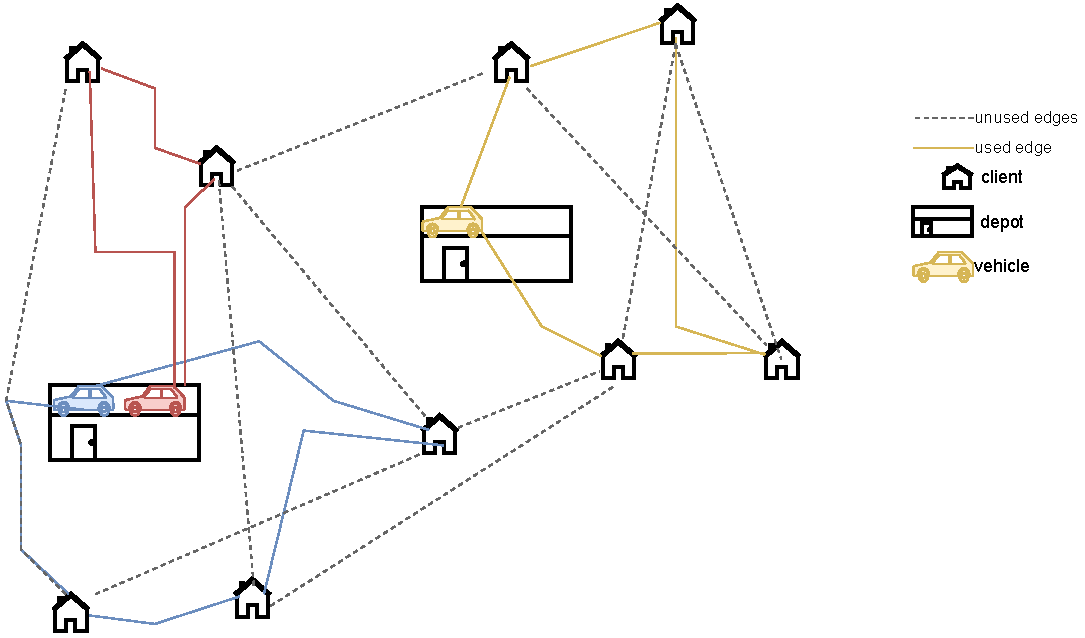
\includegraphics[height=0.85\textheight, keepaspectratio]{vrp.pdf}
	\end{center}}
\only<3>{
	\begin{columns}[T]
	\column{0.45\textwidth}
		base description
		\begin{itemize}
			\item clients need to be served
			\item cost between locations
			\item vehicles stationed at depot(s)
			\item routes need to start/end at the depot
			\item minimize cost
		\end{itemize}
	\column{0.45\textwidth}
		variants
		\begin{itemize}
		\item capacities: CVPR
		\item time windows: VRPTW
		\item pickup+delivery
		\item shifts, max route length, overtime...
		\item multi depots
		\item heterogeneous fleet
		\item reloading, multi-trip
		\item optional clients / price collection
		\item soft objectives
		\end{itemize}
	\end{columns}
}
\end{frame}


\section{Ex6 - SAT \& CP-SAT}

\begin{frame}[t]{6a: CDCL}
	\begin{block}{$1\overline{2},\ 123,\ \overline{12}3,\ 12\overline{3}4,\ \overline{3}4,\ \overline{12}4,\ \overline{1}2$}
		Perform CDCL on the following formula until you have run into two conflicts or
		found the formula to be satisfied or unsatisfiable. When making a decision, prioritize
		variables with lower indices over those with higher indices, and set the variable to
		false in your decision. 
	\end{block}
	\begin{center}
		\begin{tblr}{rowsep=0pt, colspec={|c|c|c|}}
			level & literal & reason \\
			\phline
			1 & $\overline{1}$ & $\Delta$ \\
			1 & $\overline{2}$ & $1\overline{2}$ \\
			1 & $3$			   & $123$ \\
			1 & $4$			   & $12\overline{3}4$ \\
			\phline 
			\SetCell[c=3]{} SAT &&\\
		\end{tblr}
	\end{center}
\end{frame}

\begin{frame}[t]{6a: CDCL (fixed formula)}
	\begin{block}{}
		$1\overline{2},\ 123,\ \overline{12}3,\ 12\overline{3}4,\ \overline{34},\ \overline{12}4,\ \overline{1}2,$ \only<3,4>{$\quad \underline{1},$}
	\end{block}
	\begin{center}
		\begin{columns}[T]
			\column{0.3\textwidth}
			\only<2,3,4>{
				\begin{tblr}{rowsep=0pt, colspec={|c|c|c|}}
					level & literal & reason \\
					\phline
					1 & $\overline{1}$	& $\Delta$ \\
					1 & $\overline{2}$	& $1\overline{2}$ \\
					1 & $3$				& $123$ \\
					1 & $\overline{4}$	& $\overline{34}$ \\
					1*& $4$				& $12\overline{3}4$ \\
					\phline
					\SetCell[c=3]{} $12\overline{3}4 \diamond_4 \overline{34} = 12\overline{3}$ &&\\
					\SetCell[c=3]{}	$12\overline{3} \diamond_3 123 = 12$ &&\\
					\SetCell[c=3]{}	$12 \diamond_2 1\overline{2} = 1$ &&\\
				\end{tblr}
			}
			\column{0.3\textwidth}
			\only<4>{
				\begin{tblr}{rowsep=0pt, colspec={|c|c|c|}}
					level & literal & reason \\
					\phline
					0 & $1$				& $1$ \\
					0 & $2$				& $\overline{1}2$ \\
					0 & $3$				& $\overline{12}3$ \\
					0 & $\overline{4}$	& $\overline{34}$ \\
					0* & $4$			& $\overline{12}4$ \\
					\phline
					\SetCell[c=3]{} $\overline{12}4 \diamond_4 \overline{34} = \overline{123}$ &&\\
					\SetCell[c=3]{} $\overline{123} \diamond_3 \overline{12}3 = \overline{12}$ &&\\
					\SetCell[c=3]{} $\overline{12} \diamond_2 \overline{1}2 = \overline{1}$ &&\\
					\SetCell[c=3]{} $\overline{1} \diamond_1 1 = \bot$ &&\\
				\end{tblr}
			}
		
		\end{columns}
	\end{center}
\end{frame}

\begin{frame}[t]{6b: Integer Variables and VSIDS}
	\begin{block}{}
		Why is branching by the VSIDS (SAT decision) heuristic alone not sufficient to reach a complete solution in CP-SAT? What mechanism closes the gap?
	\end{block}
	\begin{columns}[T]
		\column{0.45\textwidth}
		\only<2,3>{
			Problem:
			\begin{itemize} 
				\item VSIDS: choose highest scoring variable for branching
				\item CP-SAT integers: Order abstraction (vars for $x\leq k$ and $x=k$)
				\item CP-SAT encoding boolean literals lazily created
				\item required: exact assignment
				\item but: solver works on abstraction
			\end{itemize}
		}
		\column{0.45\textwidth}
		\only<3>{
			Solution:
			\begin{itemize} 
				\item SAT branching: decides all existing literals (ex: $\overline{x\leq2} \land x\leq7$)
				\item result: interval info (ex: $x \in [3;7]$)
				\item abstraction refinement required \\$\implies$ create new literals (ex: $x\leq5$)
				\item different refinement ideas (min-first / max-first, propagation, \dots)
				\item resolve, until every variable is fixed
			\end{itemize}
		}
	 
	\end{columns}
\end{frame}
\part{2}
\begin{frame}[highlight]{Exam}
	\begin{columns}
		\column{0.6\textwidth}
		\begin{itemize}
			\item place: SN 19.1
			\item time: July 30th, 12:30-14:30 - be there 12:15!
			\item permitted aids: Dictionary (any $\leftrightarrow$ german)
			\item required: black/blue permanent pen, ruler
			\item language: \textbf{german} (legally required, as far as we know)
		\end{itemize}
	\end{columns}
\end{frame}
\end{document}
